\chapter{技巧}
%\cleardoublepage
\section{无敌的读入优化}
\inputminted{cpp}{\source/hints/input-acceleration.cpp}
\section{真正释放STL内存}
\inputminted{cpp}{\source/hints/STL-memory-release.cpp}
\section{梅森旋转算法}
\inputminted{cpp}{\source/hints/mersenne-twister.cpp}
\section{蔡勒公式}
\inputminted{cpp}{\source/hints/zeller.cpp}
\section{开栈}
\inputminted{cpp}{\source/hints/openstack.cpp}
\section{Size为k的子集}
\inputminted{cpp}{\source/hints/subset-of-size-k.cpp}
\section{长方体表面两点最短距离}
\inputminted{cpp}{\source/hints/长方体表面两点最短距离.cpp}
\section{经纬度求球面最短距离}
\inputminted{cpp}{\source/hints/经纬度求球面最短距离.cpp}
\section{32-bit/64-bit随机素数}
\begin{tabular}{|l|l|}
	\hline
	\texttt{32-bit} & \texttt{64-bit} \\
	\hline
	73550053 & 1249292846855685773 \\
	\hline
	148898719 & 1701750434419805569 \\
	\hline
	189560747 & 3605499878424114901 \\
	\hline
	459874703 & 5648316673387803781 \\
	\hline
	1202316001 & 6125342570814357977 \\
	\hline
	1431183547 & 6215155308775851301 \\
	\hline
	1438011109 & 6294606778040623451 \\
	\hline
	1538762023 & 6347330550446020547 \\
	\hline
	1557944263 & 7429632924303725207 \\
	\hline
	1981315913 & 8524720079480389849 \\
	\hline
\end{tabular}

\section{NTT 素数及其原根}
\begin{tabular}{|l|l|}
	\hline
	\texttt{Prime} & \texttt{Primitive root} \\
	\hline
	1053818881 & 7 \\
	\hline
	1051721729 & 6 \\
	\hline
	1045430273 & 3 \\
	\hline
	1012924417 & 5 \\
	\hline
	1007681537 & 3 \\
	\hline
\end{tabular}

\section{Formulas}
\input{\source/hints/Formula.tex}
\includepdf[pages={1-2}]{\source/hints/Integral.pdf}

\section{Java}
\inputminted{java}{\source/hints/template.java}
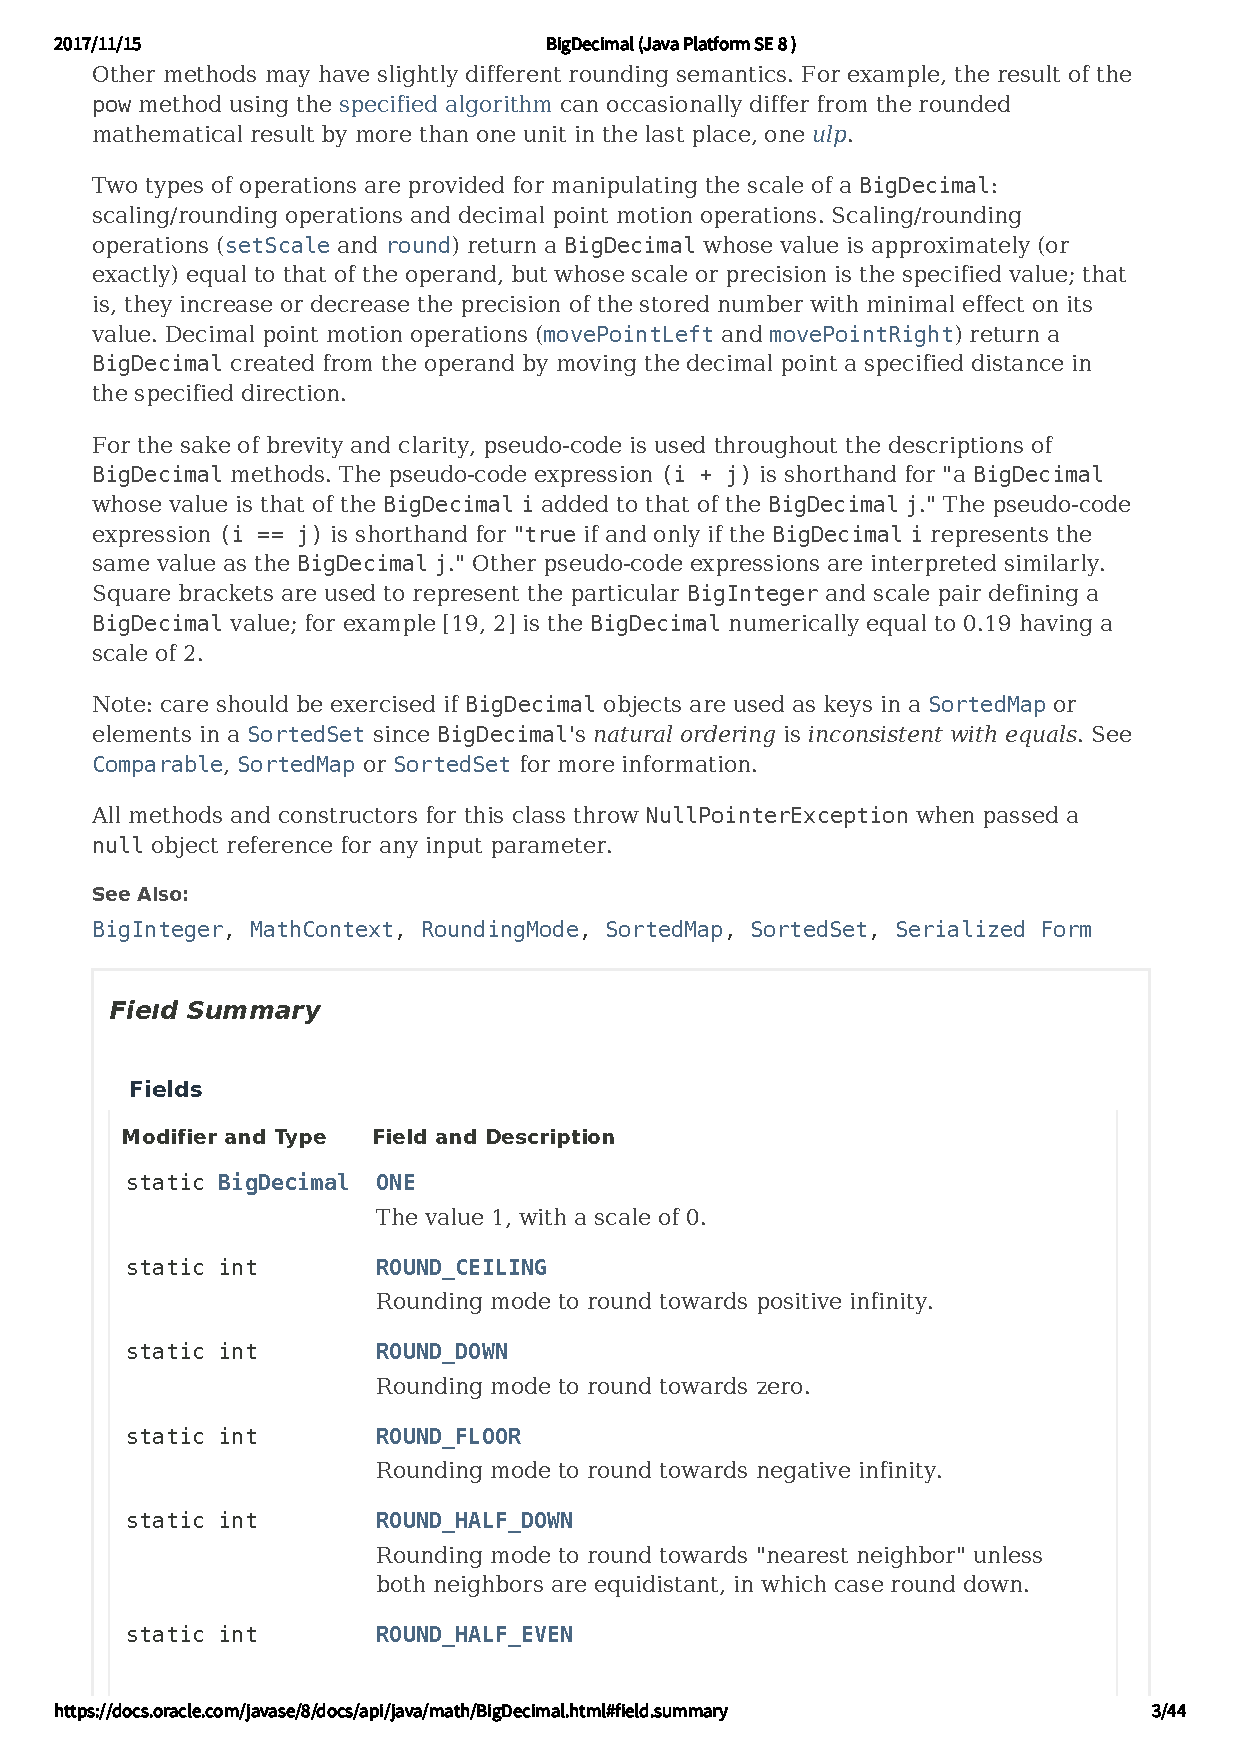
\includepdf[pages={1-6}]{\source/hints/BigDecimal.pdf}
\includepdf[pages={1-5}]{\source/hints/treemap.pdf}